\chapter{Voedselketens}\label{ch:g3:food-chains}

Gras groeit in de wei. Een sprinkhaan eet het gras. Een hagedis vangt
de sprinkhaan. Een buizerd, hoog rondcirkelend, pakt de hagedis. Vier
maaltijden --- en opeens hangt de middag van de buizerd af van hoe
groen het gras gegroeid is. De maaltijden in de natuur haken aan elkaar
tot ketens, en die leren lezen is leren hoe een hele wei samenhangt.

\section{Een voedselketen lezen en schrijven}

\begin{definition}[Voedselketen]\label{def:g3:food-chains:chain}
Een \emph{voedselketen}\index{voedselketen} is een rij levende wezens
waarin elk door het volgende gegeten wordt. Je schrijft haar met
pijlen, waarbij elke pijl \emph{``wordt gegeten door''}\index{wordt gegeten door}
betekent:
\[
\text{gras} \longrightarrow \text{sprinkhaan}
\longrightarrow \text{hagedis} \longrightarrow \text{buizerd}.
\]
Elk \omterm{def:g1:living-or-not:living}{levend wezen} is een \emph{schakel}\index{schakel} van de keten.
\end{definition}

\begin{remark}[Let op de richting van de pijl]\label{rem:g3:food-chains:arrow}
De pijl wijst van de gegetene naar de eter --- hij volgt het voedsel.
``Gras $\rightarrow$ sprinkhaan'' lees je als ``gras \omterm{def:g3:food-chains:chain}{wordt gegeten door}
de sprinkhaan''. De pijlen andersom schrijven --- naar de maaltijd toe
--- is de meest voorkomende fout bij \omterm{def:g3:food-chains:chain}{voedselketens}; onthoud dat de pijl
laat zien waar het voedsel \emph{heen gaat}.
\end{remark}

\begin{proposition}[Elke keten begint met een plant]\label{prop:g3:food-chains:start}
De eerste schakel van een \omterm{def:g3:food-chains:chain}{voedselketen} is altijd een \omterm{def:g1:plants-around-us:plant}{plant} (of een
ander \omterm{def:g1:living-or-not:living}{levend wezen} dat zijn eigen voedsel maakt). Alleen \omterm{def:g1:plants-around-us:plant}{planten} voeden
zich zonder iemand te eten --- uit licht, water en lucht, zoals
\cref{def:g1:plants-around-us:plant} zei. Elke dierlijke schakel leeft,
rechtstreeks of via anderen, van die eerste groene schakel.
\end{proposition}
\admitted

\begin{example}[Ketens uit drie leefgebieden]\label{ex:g3:food-chains:three}
In de vijver: waterplanten $\rightarrow$ donderpad $\rightarrow$
libellenlarve $\rightarrow$ stekelbaars $\rightarrow$ reiger. In het
bos: eikenbladeren $\rightarrow$ \omterm{ex:g2:animals-grow-up:butterfly}{rups} $\rightarrow$ pimpelmees
$\rightarrow$ sperwer. In de tuin: sla $\rightarrow$ slak
$\rightarrow$ egel. Eerste schakel: altijd groen.
\end{example}

\begin{omfigure}
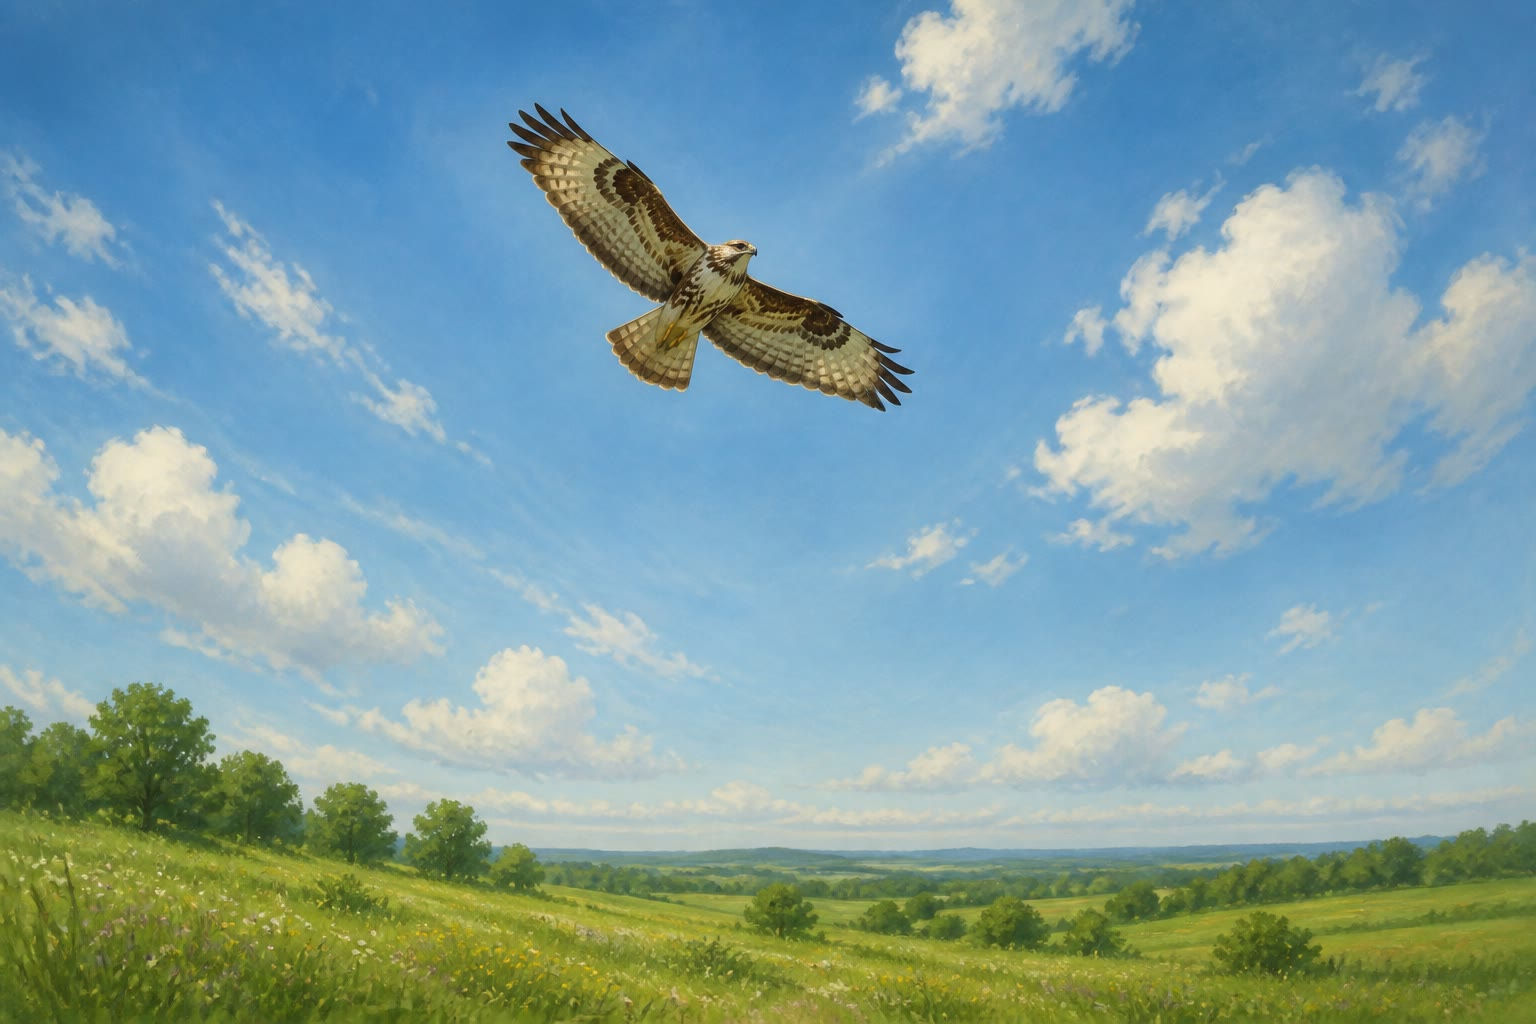
\includegraphics[width=0.6\linewidth]{images/book1/ai/g3-chains-buzzard.jpg}

{\small De laatste schakel van de weiketen op patrouille: de middag van
de buizerd hangt, drie schakels lager, af van hoe groen het gras
gegroeid is.}
\end{omfigure}

\begin{method}[Een voedselketen bouwen]\label{met:g3:food-chains:build}
\begin{enumerate}
  \item Kies een \omterm{def:g1:animals-around-us:animal}{dier} en vraag: wat eet het? Schrijf het voedsel
        links ervan, met de pijl naar de eter;
  \item stel dezelfde vraag over het voedsel, en ga naar links door tot
        je bij een \omterm{def:g1:plants-around-us:plant}{plant} komt;
  \item vraag: wie eet mijn beginnende \omterm{def:g1:animals-around-us:animal}{dier}? Breid naar rechts uit
        zolang er een eter is;
  \item controleer of elke pijl \omterm{def:g3:food-chains:chain}{``wordt gegeten door''} zegt --- met het
        voedsel dat naar rechts stroomt.
\end{enumerate}
\end{method}

\section{Als een schakel verandert}

\begin{proposition}[Schakels hangen van elkaar af]\label{prop:g3:food-chains:depend}
In een \omterm{def:g3:food-chains:chain}{voedselketen} hangt elke schakel af van de schakels ervoor, en
voedt hij de schakels erna. Als één schakel schaars wordt, lijden de
volgende schakels honger --- en de schakel \emph{ervoor}, die minder
opgegeten wordt, kan zich juist vermeerderen. Een verandering in één
schakel reist door de hele keten.
\end{proposition}
\admitted

\begin{example}[De droge zomer]\label{ex:g3:food-chains:dry}
Een droogte maakt het weidegras bruin. Sprinkhanen, met te weinig
voedsel, worden zeldzaam; de hagedissen die op ze jaagden lijden honger
en voeden op hun beurt de buizerd slecht. Eén bruine eerste schakel, en
de hele keten erboven wordt dunner --- de buizerd heeft nooit gras
gegeten, en toch voelt hij de droogte.
\end{example}

\begin{example}[De jager weghalen]\label{ex:g3:food-chains:hunter}
Stel dat de buizerds uit het dal verdwijnen. Hagedissen, minder
bejaagd, vermeerderen zich; sprinkhanen worden dan harder opgegeten en
worden schaars; het gras, minder afgeknabbeld, kan zelfs dichter
worden. Ook het weghalen van de \emph{laatste} schakel reist door de
keten --- de andere kant op.
\end{example}

\begin{remark}[Echte weiden zijn webben]\label{rem:g3:food-chains:web}
Onze keten is één enkele draad, maar de buizerd pakt ook muizen, de
hagedis eet ook vliegen, en het gras voedt ook konijnen. Veel elkaar
kruisende ketens vormen een net --- het \emph{voedselweb} dat een later
jaar zal bestuderen (\cref{ch:g2:what-animals-eat} zinspeelde er al op
met de vos, het konijn en het gras). Eerst de ketens: het zijn de
draden waaruit het net geweven is.
\end{remark}

\section{Oefeningen}

\begin{exercise}[$\star$]\label{exo:g3:food-chains:1}
Wat betekent de pijl van een \omterm{def:g3:food-chains:chain}{voedselketen}? Welke kant wijst hij op?
\end{exercise}

\begin{exercise}[$\star$]\label{exo:g3:food-chains:2}
Wat voor \omterm{def:g1:living-or-not:living}{levend wezen} is altijd de eerste schakel? Waarom?
\end{exercise}

\begin{exercise}[$\star$]\label{exo:g3:food-chains:3}
Schrijf de weiketen uit dit hoofdstuk op met haar vier schakels en haar
pijlen.
\end{exercise}

\begin{exercise}[$\star$]\label{exo:g3:food-chains:4}
Verbeter deze keten: vos $\rightarrow$ konijn $\rightarrow$ gras.
\end{exercise}

\begin{exercise}[$\star$]\label{exo:g3:food-chains:5}
Bouw een keten uit deze schakels: pimpelmees, eikenbladeren, sperwer,
\omterm{ex:g2:animals-grow-up:butterfly}{rups}.
\end{exercise}

\begin{exercise}[$\star$]\label{exo:g3:food-chains:6}
Wie wordt in de tuinketen sla $\rightarrow$ slak $\rightarrow$ egel
door de slak gegeten? Wie eet de slak?
\end{exercise}

\begin{exercise}[$\star$]\label{exo:g3:food-chains:7}
Maak met \cref{met:g3:food-chains:build} een keten van minstens drie
schakels die op de reiger van de vijver eindigt.
\end{exercise}

\begin{exercise}[$\star$]\label{exo:g3:food-chains:8}
Waarom lijdt de buizerd in de droge zomer van
\cref{ex:g3:food-chains:dry}, terwijl hij nooit gras eet?
\end{exercise}

\begin{exercise}[$\star\star$]\label{exo:g3:food-chains:9}
Tuinders die elke slak vergiftigen raken soms hun egel kwijt --- en
komen daarna \emph{meer} naaktslakken en slakken tegen dan eerst. Leg
allebei de helften uit met \cref{prop:g3:food-chains:depend}.
\end{exercise}

\begin{exercise}[$\star\star$]\label{exo:g3:food-chains:10}
``De hagedis hangt af van het gras.'' Waar of niet waar? Verdedig je
antwoord met de weiketen --- en zeg in welke richting het mislukken van
het gras reist.
\end{exercise}
